% paper.tex - IEEEtran (journal), targeting IEEE Transactions on Computers.
% Build: pdflatex paper && bibtex paper && pdflatex paper && pdflatex paper
%
% Plan of record: docs/tc_plan.md. TC rules that shape this file:
%   regular paper 10-12 double-column pages (hard max 14 with MOPC);
%   page count includes references AND biography; references capped at 45;
%   abstract 100-200 words; supplement is a separate file with no page limit.
%
% Two substantive changes from the previous version:
%   1. Mode A is no longer called a causality violation. The acknowledgment-referenced
%      span is not a causal chain: the broker's append precedes both the producer's
%      receipt of the acknowledgment and the consumer's receipt of the record, and
%      neither precedes the other. scripts/recount_spans.py settles it on the corpus --
%      the send-referenced span, which IS a chain, never inverts.
%   2. Every proportion carries a Wilson interval and every ratio a two-proportion z,
%      both emitted from the artifacts by scripts/stat_intervals.py.

\documentclass[10pt,journal]{IEEEtran}

% T1 output encoding. Under the OT1 default an accented glyph is composed rather than
% encoded, so \'e in Qu\'ema and Universit\'e renders correctly and extracts as mojibake,
% which breaks copy-paste, indexing and citation linking in the PDF IEEE receives.
\usepackage[T1]{fontenc}
% ...and the ToUnicode CMap that makes the encoded glyph extractable. T1 alone leaves the
% acute encoded but unmapped, so pdftotext returns U+FFFD. pdfTeX will build the map.
\input{glyphtounicode}
\pdfgentounicode=1
\usepackage{booktabs}
\usepackage{multirow}
\usepackage{graphicx}
\usepackage{amsmath}
\usepackage[hidelinks]{hyperref}
\def\UrlBreaks{\do\/\do\-\do\_\do\.\do\=\do\&\do\?\do\(\do\)}
% A monospace span TeX is allowed to break, for identifiers too long for a two-column
% measure. `\texttt{TimeUnit.MILLISECONDS.toMicros}` is one unbreakable word to TeX, so the
% line holding it gets stretched instead -- fifteen lines in this document reached badness
% 10000 that way before round 40 gated it, six of them in one paragraph of Section IV-A.
%
% Built on url's breaking machinery rather than on \sloppy or on hand-placed \allowbreak:
% \UrlBreaks above already lists the characters an identifier may break after, so one
% declaration reuses it and the next long name needs no thought. Not seqsplit, which breaks
% mid-word and would hyphenate `MILLISECONDS` in the middle.
\DeclareUrlCommand\brk{\urlstyle{tt}}

\newcommand{\kafka}{Kafka}
\newcommand{\redis}{Redis}
\newcommand{\tti}{TTI}

% Campaign counts, span counts and interval estimates, all derived from the committed
% artifacts by scripts/emit_paper_numbers.py rather than typed here. They were once
% written out by hand in eleven places and went stale in all eleven at once. A paper
% arguing that benchmarks misreport their own sample counts cannot afford to.
% Generated by scripts/emit_paper_numbers.py from the campaign ledger.
% Do not edit by hand -- run the script and commit the result.
% Every number below is recomputed from docs/results/external_campaigns_index.csv.
\newcommand{\ombRuns}{215}
\newcommand{\ombDiscarded}{11{,}207{,}668}
\newcommand{\ombKept}{12{,}155{,}820}
\newcommand{\ombNegatives}{41{,}403}
\newcommand{\ombKafkaDiscarded}{10{,}588{,}439}
\newcommand{\ombKafkaNegatives}{0}
\newcommand{\ombRedisDiscarded}{619{,}229}
\newcommand{\ombRedisNegatives}{41{,}403}
\newcommand{\ombRetentionMin}{0.00}
\newcommand{\ombRetentionMax}{100.00}


% Float packing. The class defaults forbid a page from being more than 80% float and a top
% float from exceeding 70% of the column, which on the two pages carrying a full-width
% figure pushed text off the page rather than setting it alongside. These change how floats
% and text share a page; the geometry, type size and leading are the class's own.
\renewcommand{\topfraction}{0.92}
\renewcommand{\bottomfraction}{0.75}
\renewcommand{\textfraction}{0.08}
\renewcommand{\floatpagefraction}{0.80}

\begin{document}

% The title carries the paper's own retraction, which is why it is phrased this way. Nothing
% in the corpus arrived before it was sent; the SUBTRACTION said so. A title claiming the
% first would reinstate the claim Section V withdraws, and "according to the arithmetic" is
% what keeps the joke on the right side of it. "Arithmetic" is also load-bearing twice over:
% Mode B's deletion is arithmetic the operator never sees, so one word carries both failures.
% "A streaming benchmark", singular: the deletion law is demonstrated on one benchmark and
% reproduced in one harness, and the plural the title used to carry was the last place in the
% paper that claimed more than that.
% v4.1 (2026-09-08): the second author's postscript asked for a shorter, cleaner title and
% proposed this one; "Artifacts" is the journal's American spelling of his British one.
\title{Faster-than-Light: Latency Measurement Artifacts in Streaming Benchmarks}

\author{Gustavo~Pedro~Ricou~and~Romaric~Duvignau%
\thanks{G.~P.~Ricou is with the School of Computer Science and Statistics, Trinity
College Dublin, Dublin~2, Ireland. E-mail: pedrorig@tcd.ie.}%
\thanks{R.~Duvignau is with the Department of Computer Science and Engineering, Chalmers
University of Technology, Gothenburg, Sweden. E-mail: duvignau@chalmers.se.}}

% Two authors, so the running head names both. IEEEtran's \MakeLowercase{\textit{et al.}}
% is for three or more; it read "Ricou et al." while the paper had four names.
\markboth{IEEE Transactions on Computers}%
{Ricou and Duvignau: Faster-than-Light}
\maketitle

% Standard shape, in order: context; problem; method; quantitative results; implication. No
% term of the paper's own appears before the problem is stated, and the two findings are
% given in the field's words (timestamp, delivery, resolution) rather than in ours.
\begin{abstract}
Message-broker benchmarks now compare systems on sub-millisecond paths, where the delivery
measured is shorter than the delays and resolution of the timestamps that measure it. A
widely used benchmark misreports in two ways that leave no trace. First, a
latency computed from two timestamps written by different threads is negative whenever the
thread writing the reference timestamp is scheduled late by more than the delivery. A
per-run sign check rejected $\auditRejected$ of $\auditRuns$ runs; referenced to the
send timestamp the same events never invert on one clock over $\spanEvents$ events, so
the cause is
scheduling, not clock synchronization; real-time priority on the timestamping threads cuts
the negative rate $\rtFactorLow$--$\rtFactorHigh\times$ at unchanged utilization.
Second, the benchmark keeps an end-to-end sample only when its millisecond-resolution
latency is strictly positive and does not count what it discards: of $\ombMedianCells$
embedded-mode cells whose summary we captured, $\ombGridMedianCells$ reported a median that was an exact
multiple of one millisecond, computed from $\ombGridRetentionMin$--$\ombGridRetentionMax\%$
of the samples taken. We identify and experimentally characterize both --- with an exact
identity for the negative span, a pre-registered manipulation, and an audit of
\harnessAuditedWord{} tools --- show that they materially alter reported results, and derive
checks benchmark authors can apply.
\end{abstract}

% Alphabetical, case-insensitively, and gated by test_index_terms_are_alphabetical.
% One entry carries an initial capital: it is a taxonomy string quoted verbatim from the IEEE
% Computer Society subject list, where it appears that way. The others are ordinary noun
% phrases. The mixture is deliberate, and lower-casing the taxonomy term would stop it
% matching the taxonomy.
% Round 33's referee asked for uniform case and the request is declined on the grounds above:
% the capital is the quotation mark. Recorded here so a later round does not raise it again,
% and note that a comment *inside* the block below is parsed as two index terms by
% test_index_terms_are_alphabetical -- which is how this note ended up outside it.
\begin{IEEEkeywords}
distributed systems;
measurement techniques;
measurement, evaluation, modeling, simulation of multiple-processor systems;
message passing;
performance attributes;
scheduling and task partitioning.
\end{IEEEkeywords}

\IEEEpeerreviewmaketitle

\section{Introduction}
\label{sec:intro}

% The two figures sit here in the source and float to the top of page 2. Their definitions
% are in Section II, which begins on that page; a reader who is not a scheduling specialist
% meets the picture before any claim about it, which a co-author required, and meets its
% definitions beside it, which another did.
\begin{figure*}[t]
\centering
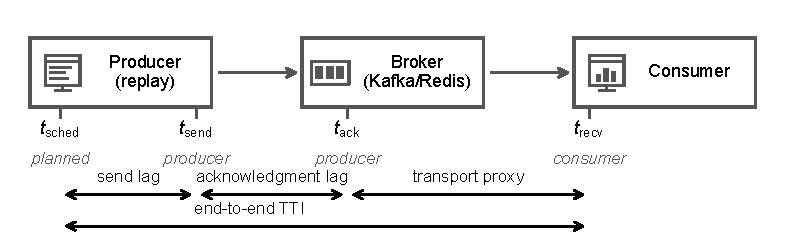
\includegraphics[width=\textwidth]{docs/results/figures/pipeline_schematic.pdf}
\caption{\textbf{System measured, and where its clocks are read.} A replay process paces
recorded match events at a chosen rate into a broker --- \kafka{} or \redis{} Streams --- and
a consumer reads them back. The four timestamps and the four spans they bracket are
defined in Section~\ref{sec:sysmodel}; the upper three are the terms of
Equation~\ref{eq:tti} and sum to the fourth. The transport proxy, the span this paper is
about, subtracts a producer-process timestamp from a consumer-process one. Both
processes run on
one host reading one clock unless stated otherwise, so nothing that follows depends on
clock synchronization.}
\label{fig:pipeline}
\end{figure*}

\begin{figure*}[t]
\centering
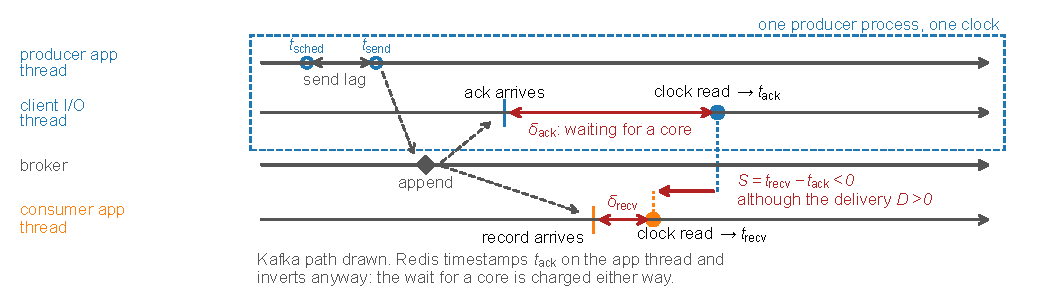
\includegraphics[width=\textwidth]{docs/results/figures/measurement_model.pdf}
\caption{\textbf{Late timestamp, not an early record.} How a positive latency is measured
as negative, on one clock. Two threads of the producer process take the two timestamps ---
the application thread calls send, the client's I/O thread runs the delivery callback ---
and whichever one timestamps must first be scheduled, so the difference inverts when the
acknowledgment's timestamping delay ($\delta_{\mathrm{ack}}$ in the drawing;
$\delta_{\mathrm{recv}}$ is the consumer's) exceeds the delivery. The path drawn is \kafka{}'s;
\redis{} has no second thread and inverts on a larger share of runs (Supplement~S16.3). The
producer's own timestamps, $t_{\mathrm{sched}}$ and $t_{\mathrm{send}}$, precede the
acknowledgment, and the span referenced to them never inverts (Table~\ref{tab:spans}).}
\label{fig:model}
\end{figure*}

\IEEEPARstart{M}{essage}-broker benchmarks inform purchasing and architecture decisions,
and the paths they compare now complete in well under a millisecond. This paper asks what can
go wrong when a benchmark measures a sub-millisecond path, and how its authors can detect or
avoid it. We answer with two concrete failure modes, each characterized by manipulation, and
with the checks they imply.

% The two figures moved to Section II, beside the paragraph that defines what they draw. The
% introduction still points at them, which is the right direction: a reader meets the picture
% two pages on, next to its definitions, rather than here, ahead of any of them.
A latency benchmark measures a message by reading a clock when the message is sent and
again when it arrives. Subtracting the two timestamps gives the measured latency.
The message does not take those readings (Fig.~\ref{fig:pipeline}); two \emph{threads} do
(Fig.~\ref{fig:model}), each of which must be scheduled onto a core before it can read the
clock, and each of which waits for that core on its own account. That wait is the
\emph{scheduling delay}\label{def:scheddelay}: the time a thread that is ready to run spends
queued before a core runs it. On a busy machine either wait can exceed the delivery being
measured. When the two waits differ by more than the
delivery, the subtraction is negative. Nothing arrived before it was sent; the two readings
were taken in the wrong order. Separately, the benchmark that the cross-broker comparison
literature shares (Section~\ref{sec:related_bench}) records its cross-process timestamps in
whole milliseconds and keeps only positive differences, so on a path faster than a
millisecond it discards samples at a rate fixed by arithmetic rather than chance. Neither
failure is visible in the benchmark's output, and both are caught by checks that cost
nothing.

% Not "one number governs both". Scheduling delay is a distribution and timestamp resolution
% is a fixed quantity; a co-author found the shared-number framing forced, and the safer
% statement is the one below: each becomes a problem when the delivery approaches its own
% timescale. What survives of the old paragraph is the point that the binding delay is not
% the one a specification discloses.
Both failures arise when the delivery being measured approaches the timescales of the
measurement mechanism. Scheduling delay is a distribution and timestamp resolution is a
fixed quantity, and they act differently: on the one axis they share, only one of the two
can be escaped (Supplement~S9). Sub-millisecond broker paths are where each
becomes comparable to the delivery for tooling in current use. Where that happens is not
where a specification says. The timestamp resolution is one millisecond, but the delay that
binds is the scheduler's: the last mode of the run-queue stall distribution sits in the
$\tracedModeLo$--$\tracedModeHi$~ms bucket, on the scheduler's derived $\baseSliceMs$~ms base
slice (Section~\ref{sec:tail}), three times the timestamp resolution and nothing a
specification discloses.

\subsection{Contributions}

% The standard form, and only words already defined above it. The evidence behind each
% item -- denominators, the spread statistic, the grid -- is stated where it is shown, in
% Sections IV and V, not here; a co-author counted seven undefined terms in the previous
% version of this list.
We make three contributions, each established by manipulation rather than by observation
alone.
\begin{enumerate}
\item \textbf{An exact account of the negative latency, on one clock}
(Section~\ref{sec:mechanism}). The acknowledgment-referenced span is the delivery less the
acknowledgment lag, $S = D - A$ per event. A negative value is therefore an ordering between
two measured quantities and not a fault in either clock. Four manipulations separate scheduling
from its rival explanations, and the send-referenced span over the same $\spanEvents$
events never inverts.
\item \textbf{What a positivity filter costs a reported distribution}
(Sections~\ref{sec:external} and~\ref{sec:tools}). The fraction of samples a millisecond-resolution benchmark
retains is fixed by the ratio of the delivery to the timestamp resolution --- arithmetic a
1970 counter manual already carries~\cite{hp1970tia}. New is its consequence under silent
deletion: that fraction decides the distribution the benchmark reports, is never shown to
the operator, and a pre-registered manipulation of message size moves a configuration
across the boundary it predicts. A source audit of \harnessAuditedWord{} tools places the
disposal in the tooling rather than in the one benchmark we measured.
\item \textbf{A per-run audit and the reporting rules it implies}
(Sections~\ref{sec:gate} and~\ref{sec:authors}). A sign check applied uniformly to all
$\auditRuns$ runs rejected $\auditRejected$, including every run behind our own first
result. Each part of the practice exists
already~\cite{paxson2004sound,specjbb2015,kistowski2015build}. What we add is their
conjunction: the rejection rate published as a headline quantity, and the rule that the
retained fraction of samples and the sign of each discard belong beside every reported
latency.
\end{enumerate}

% The chronology subsection is gone from the introduction: the order in which the work
% happened is the supplement's spine now (its S1), and an introduction that narrates its own
% history is what a co-author called "the start of the experimental story". The one sentence
% kept is the withdrawal itself, because a reader deciding whether to trust the audit should
% know it cost the authors a result; it sits in the contributions above.
% Round 54 cut the roadmap paragraph for the page budget. It asserted nothing -- it restated
% the table of contents -- and it is not the venue's habit: of the 46 readable IEEE
% Transactions on Computers papers in docs/reference_tc, 18 carry a roadmap and 28 do not.
% The section titles are descriptive since the v4 restructure, which is what a roadmap was
% standing in for.

\section{System and Measurement Model}
\label{sec:sysmodel}
\label{sec:metrics}

% Definitions live here, in the text, once, before anything is claimed about them. A
% co-author found them spread across a figure caption, the opening of Method and a
% subsection three pages on, with D introduced after S had been used and T_true before
% either. Everything a later section subtracts is named on this page. The two figures are
% placed in the source at the top of the introduction so that IEEEtran floats them onto
% page 2, which is where a second co-author asked the system to be drawn -- inside the
% first two pages -- and which is also where this section begins.
A producer process sends recorded events at a paced rate to a broker, and a consumer
process reads them back; Figure~\ref{fig:pipeline} draws that path and the timestamps taken
on it. Four timestamps bracket a message's path:
$t_{\mathrm{sched}}$, when the event was due to be sent; $t_{\mathrm{send}}$, immediately
before the send call; $t_{\mathrm{ack}}$, when the producer learns that the broker accepted
the message; and $t_{\mathrm{recv}}$, when the consumer holds the record. A fifth,
$t_{\mathrm{out}}$, is written by the consumer once it has parsed the record. The difference
$t_{\mathrm{out}} - t_{\mathrm{recv}}$ is the consumer's own handling.

Three quantities are defined from these timestamps and used throughout:
\begin{equation}
\begin{aligned}
D &\equiv t_{\mathrm{recv}} - t_{\mathrm{send}}, \qquad
A \equiv t_{\mathrm{ack}} - t_{\mathrm{send}}, \\
S &\equiv t_{\mathrm{recv}} - t_{\mathrm{ack}} \;=\; D - A .
\end{aligned}
\label{eq:model}
\end{equation}
$D$ is the \emph{delivery}, from the send call to the consumer holding the record. $A$ is
the \emph{acknowledgment lag}, from the send call to the producer observing the broker's
acknowledgment. $S$ is the span the benchmark literature reports as broker latency. We
call it the \emph{transport proxy}, for the reason given in
Section~\ref{sec:proxy}.

Two more quantities belong to the model rather than to either failure. Write $\tau$ for
the \emph{timestamp resolution} --- the \emph{quantum}, one millisecond in the benchmark of
Section~\ref{sec:external} --- and $T_{\mathrm{true}}$\label{def:ttrue} for the \emph{true
delivery} of a message. That is the interval $D$ would report if it were measured with an arbitrarily
fine timestamp, which is what $D$ measures up to the consumer's own timestamping jitter. The primary end-to-end measure is \textbf{Time-to-Insight}
(\tti{}), from scheduled emission to availability at the consumer:
\begin{equation}
\mathrm{TTI} = \underbrace{(t_{\mathrm{send}}-t_{\mathrm{sched}})}_{\text{send lag}}
             + \underbrace{A}_{\text{acknowledgment lag}}
             + \underbrace{S}_{\text{transport proxy}} ,
\label{eq:tti}
\end{equation}
which telescopes to $t_{\mathrm{recv}} - t_{\mathrm{sched}}$ (Supplement~S24 maps every
metric of the corpus onto the span it covers). The first term, the \emph{send lag}, is how
late the send call ran after the event was due, measured on the producer's own thread. A
\emph{span} is any difference of two of
these timestamps, and a \emph{negative span} is one whose difference is below zero. The
term is Sharma et al.'s~\cite{sharma2026causality}, kept for the
% Round 54: the reference left the list to pay for two Related Work sources, and the clause
% stayed. RFC 1242 is located by its number, so a reader can still check the distinction --
% which is the principle tests/unit/test_attributed_claims.py now states and holds.
observable while declining the causal reading they give it. It is not RFC~1242's negative
latency, a cut-through forwarding artifact. \emph{Retention} is the
fraction of the samples a measurement tool takes that survive into what it reports, not
\kafka{}'s log-retention setting.

\subsection{The transport proxy is not a causal chain}
\label{sec:proxy}
\label{sec:model}
This distinction decides everything that follows. $D$ and \tti{} are genuine chains: the
producer sends, the broker appends, the consumer receives, and each event precedes the
next. $S$ is not. It subtracts the producer's receipt of the broker's acknowledgment from
the consumer's receipt of the record. The broker's append precedes both of those events,
but neither of them precedes the other: they are two branches of one cause. The
acknowledgment timestamp is therefore a \emph{late, producer-side observation} of a
broker-side event, and $S$ is a proxy for the delivery rather than a measurement of it.

Since Equation~\ref{eq:model} is an identity holding per event, and whatever the signs,
\begin{equation}
S < 0 \quad\text{if and only if}\quad A > D ,
\label{eq:negspan}
\end{equation}
so the span is negative exactly when the acknowledgment lag exceeds the delivery. That is
an identity, not a model: both sides count $\spanNegAck$ negatives over the
$\diseaseEvents$ events of our corpus, and the build fails if they part. Reading it as a
lag outrunning a delivery does need both to be non-negative, and both are measured rather
than assumed: $D$ and $A$ are the two send-referenced chains of Table~\ref{tab:spans}, and
neither inverts on any event. Every timestamp is
written some time after the event it marks, because the thread that reads the clock must
first be scheduled (Fig.~\ref{fig:model}). This is not the cost of the clock call, which is
small and separately measurable~\cite{kuperberg2011timers}, but the delay before the call
runs at all. Only the difference of two such delays matters. When the acknowledgment
branch is delayed by more than the delivery, $S$ is negative with nothing physically
impossible having occurred.

% The wording a co-author asked for, and the one used everywhere the negativity is
% discussed: a negative S does not show a timestamp is wrong; it shows the acknowledgment
% cannot serve as the origin of a non-negative delivery latency.
What a negative $S$ establishes is precise and limited. It does not show that either
timestamp is wrong: $t_{\mathrm{ack}}$ may record exactly when the producer observed the
acknowledgment. It shows that the acknowledgment cannot serve as the origin of a
non-negative delivery latency for that event. That is the use the benchmark literature
puts it to. The negative-span rate is therefore a property of the quantity being measured,
not only of the machine. A fixed distribution of $A$ overlaps a small $D$ almost entirely
and a large one hardly at all. That is why a configuration whose transport runs to tens of
seconds passes every run while the same hardware measuring one millisecond fails
wholesale.

\section{Background and Related Work}
\label{sec:related}

That measurement error can dominate a benchmark is established; what prior work does not
supply is a check applied to every run, and a count of what the check removes.

\subsection{Streaming benchmarks}
\label{sec:related_bench}
Broker comparisons appear continuously, in peer-reviewed venues and in the gray
literature. Apache \kafka{} and \redis{} Streams are the pair they most often name,
and the OpenMessaging Benchmark~\cite{openmessaging2018} is the tool they share. That
experimental setup can dominate a result is established~\cite{mytkowicz2009wrong}, and how
to report one is a settled literature we
follow~\cite{georges2007rigorous,hoefler2015benchmarking}. What that literature does not do
is check what its tool discards. Where a comparison reports a median above the
tool's one-millisecond timestamp resolution, the deletion arithmetic of
% Round 55 moved the denominator to Supplement S33.4, where the exhibits are set out. With
% two comparisons it read against its own sentence: the count said both had been placed
% against the resolution, and the clause after it said one of them cannot be placed at all.
% The exhibit is the argument; the count is bookkeeping and belongs beside the bookkeeping.
Section~\ref{sec:external} does not bind. Not every comparison does: a 2026 comparison
names a percentile for a single broker and gives the other two only
``sub-millisecond''~\cite{indexdev2026brokers}, so its ranking cannot be placed against that
resolution at all.

The tools are few and shared, so a defect in one is not one project's problem. The audit of
Section~\ref{sec:tools} reads \harnessAuditedWord{} tools at source and finds
\harnessSilentWord{} disposing of inverted samples without counting them. Coarse timestamp
resolution reaches further than the disposal does: the end-to-end tool bundled with Apache \kafka{}
itself computes its percentiles from millisecond-truncated integers~\cite{kafka_tools}. The
architecture that produces those spans is not a blunder to be
designed away: a producer that blocked for each acknowledgment could not generate load at
all. What a benchmark can drop is the habit of subtracting two such timestamps without
checking the sign of the result.

That literature already stands its clocks carefully: Karimov et
al.~\cite{karimov2018benchmarking} separate event-time from processing-time latency, and
Van~Dongen and Van~den~Poel~\cite{vandongen2020evaluation} use single-broker append
timestamps ``to ensure correct latency measurements'' --- our one-clock rule, arrived at
independently. Neither asks what a millisecond timestamp does to a sub-millisecond path, nor
checks which samples the tool keeps; those two questions are this paper.

\subsection{Cross-process time measurement}
\label{sec:related_time}
Lamport~\cite{lamport1978time} established that a distributed system has no single physical
time, only a causal partial order. That order decides this paper's central span. An
acknowledgment at the producer and a record at the consumer are two branches from the
broker's append, and neither precedes the other. Measurement systems defeat clock
disagreement~\cite{ieee1588} by calibrating cross-node counters~\cite{yang2022cloudprofiler},
timestamping in the NIC~\cite{kogias2019lancet} or the switch dataplane~\cite{kundel2024p4sta},
and measuring the timer's own accuracy~\cite{kuperberg2011timers}.

One prior result bounds our claim closely. Villain et al.~\cite{villain2012probing},
profiling FreeBSD against a DAG hardware reference, found the outgoing socket timestamp
``does not respect causality'' --- packets leave before the timestamp meant to mark their
departure is written --- under every stress pattern including none. They attribute host
latency to interrupt processing, scheduling and context switching. That is the scheduling
mechanism studied in Section~\ref{sec:mechanism}, published in 2012 and measured more
precisely than we measure it. What it does not give, and we add, is its consequence for a
two-process measurement: the negative-span rate falls as the delivery being measured
grows. The manipulations that establish it separate scheduling from its rival
explanations (Section~\ref{sec:twostate}). The audit half has its own ancestor.
Paxson~\cite{paxson1998calibrating} treated physically impossible transit times as
measurement failure and published the proportion of traces affected.
Lancet~\cite{kogias2019lancet}, a latency-measurement tool that timestamps in the network
interface, is the nearest existing gate: it tests each run's samples for statistical
stability and reports an inconclusive verdict when they fail, where we decline to publish
at all. Neither reports the fraction of runs a campaign lost.

Production tracing reached the same answer without a mechanism: skew adjusters that rewrite
a span's timestamps are called harmful and have defaulted to off since
2020~\cite{jaeger_harmful}, and nobody had measured how much such a correction moves.

Swami and Chougule~\cite{swami2026observability} state the wider position concurrently,
that timing observability is itself an interference-sensitive resource; their reference is
a logic analyzer outside the system, ours the sign of a subtraction inside it.

Sharma et al.~\cite{sharma2026causality} reach the same observable by another route: they
count negative timing spans in distributed inference systems
and propose a \brk{causality_health} check. Injecting skew, they see no violations up to
$3$~ms and clear ones by $5$~ms, and read that as a skew threshold. We take their term, and
dispute the reading rather than their measurements. They hold that ``queueing alone cannot
produce negative timing spans''. For the queue they model, backlog at a service stage, we
agree. A \emph{second} queue decides ours: the run queue the timestamping thread waits in
for a CPU. We see rates near $23\%$ at $88\%$ utilization on one host, with an inter-host
offset of $\interHostOffsetMs$~ms where two are used. We move that rate fiftyfold without
touching a clock. A threshold in milliseconds of skew does not transfer to a loaded
machine. The same attribution was offered for the benchmark we audit: asked why
publish latency could exceed end-to-end latency, a maintainer cited inter-node skew of
``\textasciitilde 100ms''~\cite{omb_issue216} and, told both processes ran on one node, called
the measurement reliable. That is the configuration our audit rejects most often.

\subsection{Resolution and discarded samples}
\label{sec:related_resolution}
That a timer coarser than the interval it measures invalidates the measurement is
textbook~\cite{kuperberg2011timers}, and older than every tool we audit. Metrology has long
carried both our failure modes in one uncertainty budget: the NIST stopwatch guide budgets
reaction time beside display resolution, and notes that at short intervals the resolution
becomes significant against the stopwatch's rated accuracy~\cite{nist2009stopwatch}. The
observation that periodic sampling commensurate with a periodic phenomenon sees only part
of it is also old: it is the IPPM framework~\cite{rfc2330}, and RFC~3432 makes a randomized start mandatory for periodic
streams~\cite{rfc3432}. Coordinated omission~\cite{tene2015latency} is the mirror image ---
there the measurement fails to record samples that would have been slow, here it deletes
samples that were fast. Millsap and Holt draw the opposite conclusion from the same
arithmetic~\cite{millsap2003oracle}: coarse timing survives in aggregate \emph{because} the
two signed errors cancel. A filter admitting only positive samples removes one sign, and
with it the cancellation that defence depends on.

The mathematics is older still and is not ours: Hewlett-Packard's Application Note
162-1~\cite{hp1970tia} carries our retention identity, the reduced fraction the grid
structure turns on, our ceiling
on resolution gain, the symptom and the cure. What is new is the
sign of the operation. HP \emph{keeps} both readings and the retained fraction \emph{is} the
estimator; the benchmark discards that population. Our contribution is not that arithmetic ---
we derived it, then found it in a counter manual --- but its consequence under deletion. A
harness released in 2018 throws away the quantity a 1970 counter measured with.

\paragraph{Sources of scheduling delay}
\label{sec:related_tail}
A runnable thread does not always run, and work-conservation violations are documented for
CFS-era schedulers~\cite{lozi2016wastedcores}, ours being EEVDF-era. Queueing gives the
leading-order account, and the core-count contrast of Table~\ref{tab:mechanism} refutes a
single-parameter law rather than queueing itself.
Chandrasekar and Kramberger~\cite{chandrasekar2026bias} apply
such a law to benchmark bias and reach our inflation half independently. We refute it on
the load axis
(Section~\ref{sec:mechanism}). What a positive number cannot show remains ours: the negative
span, and the sign channel that makes the displacement legible.

\section{Experimental Setup}
\label{sec:method}

% Split the way a co-author asked: testbeds, terms, clocks, workload, validation,
% statistics, each its own subsection. The measurement model that used to open this section
% is Section II now; what remains here is what was built and how it was run.
Everything below is measured on the system of Section~\ref{sec:sysmodel}, on one clock
unless the text says otherwise. The rule that decides which runs count was fixed before
any result was read.

\subsection{Testbeds}
\label{sec:testbeds}
Every measured finding comes from four Oracle Cloud \brk{VM.Standard.E5.Flex} instances, three
brokers and one driver. They run Ubuntu 22.04 on kernel \brk{6.8.0-1057-oracle} (EEVDF
scheduler) and CPython 3.10, on a private network. Client libraries are pinned identically,
and \texttt{chrony}-disciplined clocks are logged every minute. The producer and the consumer
run as separate \emph{processes on one host}. One early phase perturbed the measurement
enough to be unusable and is excluded from every result here. The campaigns that remain
measure utilization with no core pinning (Supplement~S1). A second testbed, a workstation
running the brokers under containers, enters only through the audit, whose rejection count
spans both (Section~\ref{sec:audit}).

\subsection{Terms}
\label{def:vocabulary}
% One paragraph, one containment, used the same way everywhere after it. A co-author found
% run, replicate, cell, arm and condition used as if interchangeable, and none of them
% defined; "arm" is retired for "configuration" because in this journal's papers "arm" is
% the processor architecture.
A \emph{condition} is one point of the experimental design: a broker, a send rate, a
message size, a background load and a consumer pattern. A \emph{cell} is a condition
together with a workload; where the workload is fixed the two coincide. The benchmark
audit of Section~\ref{sec:external} counts cells because it varies the workload. A
\emph{run} is one execution of a cell, and a \emph{replicate} is a further run of the same
cell. Where a manipulation compares settings that differ in one variable, each setting is a
\emph{configuration} of that manipulation. Utilization\label{def:rho} $\rho$ is the
fraction of CPU time busy on the host, measured over the run rather than configured. The
core count $k$\label{def:kcores} is the number of cores the background load occupies; both are
manipulated in Section~\ref{sec:mechanism}. Two settings that reach the same utilization
with the background load on different numbers of cores differ in \emph{load
geometry}\label{def:geometry}: \emph{concentrated} on few cores or \emph{spread} over many.

\subsection{Clocks}
\label{sec:clocks}
% Two separate justifications, because one sentence had been answering two questions.
% CLOCK_MONOTONIC is system-wide and comparable across processes on one host; the Time
% Stamp Counter is a per-core register; neither is the reason CLOCK_REALTIME was chosen.
Both processes read the wall clock (\brk{time.time_ns()}, \textsc{clock\_realtime}). The
two-host configurations need a common epoch, and the choice is kept on one host so that
every configuration is measured the same way. On one host \textsc{clock\_monotonic} would
have guaranteed that consecutive reads never go backwards; we forgo that exclusion and
establish it from data instead (Section~\ref{sec:mechanism}; Supplement~S15). The Time Stamp Counter (TSC) is a
per-core cycle register and a separate matter: whether the kernel's clocksource is coherent across virtual CPUs is
bounded in Section~\ref{sec:threats}. The measured inter-host offset, where two hosts are
used, is $\interHostOffsetMs$~ms.

\subsection{Workload and load generation}
\label{sec:workload}
The workload is StatsBomb's open football event data~\cite{statsbomb2023}
(CC~BY-NC-SA~4.0): per-match event streams --- passes, shots, pressure events --- with
sub-second event times. We replay $3{,}315$ matches, preserving each match's event order
and scaling its inter-event spacing to the chosen send rate. It stands for small frequent
ordered messages rather than for any particular deployment, and nothing below depends on
its content beyond message size and rate (Supplement~S20). The send schedule is measured rather than assumed.
Pacer jitter is $\pacerJitterLo$--$\pacerJitterHi\,\mu$s at p90, and the achieved rate is recorded per run against
elapsed wall time: the self-validation SPEC and TPC ask of a
benchmark~\cite{kistowski2015build}, applied to the load generator.

The two clients place one timestamp differently, and it matters to every span referenced
to $t_{\mathrm{recv}}$. \kafka{}'s client deserializes the payload before that timestamp
and \redis{}'s after it, so such a span carries one client's payload parse and not the
other's (Supplement~S16.1); Section~\ref{sec:brokers} says what that is worth.

\subsection{The consistency check}
\label{sec:gate}
We fixed the rule before the final campaign and apply it to every run, including those
whose results looked reasonable. \textbf{A run is rejected if more than $1\%$ of its events
carry a negative value in any latency component, or if the median of any component is
negative.} A condition is usable only if all of its runs survive. Where a condition is
partly rejected we report the fraction of its runs that survived. The one-per-cent figure
is a threshold, not a discovery. The supplement sweeps it from $0$ to $20\%$ and no rejected
condition becomes usable anywhere in that range, so the verdicts do not turn on where the
line was drawn (Supplement~S18).

The justification is not that a negative is impossible, because for the transport proxy it
is not (Section~\ref{sec:proxy}). It is that a negative span shows the reference
timestamp has failed as an origin for that event. A run whose reference is unusable on
more than one event in a hundred cannot report a latency, whatever the cause. The check is a \emph{necessary} condition, not a validation
procedure. A corpus that fails is unusable, and one that passes has cleared the cheapest
available bar and nothing more. We use the sign as a gate rather than as an estimator. The
same constraint supports estimation, since offset and skew can be recovered from a delay
envelope~\cite{paxson1998calibrating}. An estimator corrects a record. A gate
declines to publish from a run whose measurement demonstrably failed, and we preferred
declining.

% "A model of the failure" moved to Section II as the identity it always was. The
% probability notation that dressed S = D - A as a stochastic model went with it; the
% "invented a time zone" line, which was a joke, did not survive the move.
\subsection{Statistics}
\label{sec:stats}
Every proportion below is a count over a stated denominator with a Wilson score $95\%$
interval, not Wald: at the real-time configurations' rates the normal approximation is
shifted low and covers below its nominal rate. Holm correction is applied within a
named family, and the corrected value is the one the supplement's tables display. Tail indices are
estimated on the traced histogram by grouped maximum likelihood and by an exceedance ratio.
A slope through survival points would mislead, because the buckets are interval-censored. The
grouped estimator on log-spaced bins is Virkar and Clauset's, the Hill estimator for
binned data, and we use their bootstrap for goodness of fit~\cite{virkar2014power}. The
remaining estimators are inventoried in Supplement~S24. All interval arithmetic is
recomputed from the committed artifacts at build time
by \texttt{scripts/stat\_intervals.py} and \texttt{scripts/tail\_index\_traced.py}. The
tables reporting it are generated rather than transcribed.

% Descriptive title, not "Mode B": a co-author met "Mode B" before "Mode A" and neither
% label had been introduced. The labels are gone from the paper; the section names say what
% each failure is.
\section{Failure Mode 1: Timestamp-Reference Bias}
\label{sec:mechanism}

The negatives in our own corpus are produced by scheduling, and we establish this by moving
scheduling while holding everything else fixed.

\subsection{What the audit rejected}
\label{sec:audit}
The rule of Section~\ref{sec:gate} rejects $\auditRejectedWorkstation$ of
$\auditRunsWorkstation$ runs on the workstation testbed ($\auditPctWorkstation\%$) and
$\auditRejectedCloud$ of $\auditRunsCloud$ on the cloud testbed ($\auditPctCloud\%$), every
run behind our first result among them: on that first testbed
$\auditUsableConditionsWorkstation$ of $\auditConditionsWorkstation$ conditions survive,
which is what applying the rule to ourselves cost.

Table~\ref{tab:spans} separates the components over a wider population than the audit:
every cloud run that produced matched events, $\spanRuns$ of them, rather than the
$\auditRunsCloud$ behind a reported result. A condemned run answers which span inverts as
well as a clean one does, so none is excluded. The
acknowledgment-referenced proxy is negative on $\spanNegAck$ of $\spanEvents$ events
($\spanNegAckPct\%$; Wilson intervals are under $0.1$ points here and omitted hereafter).
Of the runs, $\spanRunsOverOnePct$ exceed the one-per-cent threshold on it. The
send-referenced span, the acknowledgment lag $A$ and \tti{} --- every causal chain the
corpus contains --- are negative on \textbf{no event at all}. None of the $\spanNegAck$ messages arrived before it was
sent; the acknowledgment timestamp was written late. The rejections are therefore evidence
that the acknowledgment cannot serve as the origin of a delivery latency on those events,
which is precisely what the check of Section~\ref{sec:gate} is for.

\textbf{The sign is a threshold, so the negatives count only the worst of the displacement.}
The acknowledgment lag exceeds half the delivery time on $\diseaseOverHalf\%$ of events and a
tenth of it on $\diseaseOverTenth\%$. The check fires only on the $\diseaseOverWhole\%$ where
it exceeds the whole. The two are correlated within a run (median $\spanRhoMedian$ over
$\spanRhoConditions$ conditions), one scheduler causing both, which suppresses crossings
without touching the displacement.
A path longer than the timestamp resolution is not clean but quiet.

\begin{table}[tb]
\caption{\textbf{Negatives by span and broker} ($\spanRuns$ runs, $\spanEvents$ events,
one clock). Only the acknowledgment-origin span inverts, and it does so under both
brokers: \kafka{} on $\spanKafkaNegAckPct\%$ of its $\spanKafkaEvents$ events,
\redis{} on $\spanRedisNegAckPct\%$ of its $\spanRedisEvents$, and the
causal chains are clean under both --- the acknowledgment lag $A$ among them, its
smallest run minimum $\spanAckLagFloorUs\,\mu$s clear of zero.}
\label{tab:spans}
\centering
\footnotesize
\setlength{\tabcolsep}{5pt}
\begin{tabular}{@{}llrrr@{}}
\toprule
Span & Origin timestamp & \kafka{} & \redis{} & All \\
\midrule
$t_{\mathrm{recv}}-t_{\mathrm{ack}}$ & acknowledgment & $\spanKafkaNegAck$ & $\spanRedisNegAck$ & $\spanNegAck$ \\
\midrule
$t_{\mathrm{recv}}-t_{\mathrm{send}}$ & send (chain) & $\spanKafkaNegSend$ & $\spanRedisNegSend$ & $\spanNegSend$ \\
$t_{\mathrm{out}}-t_{\mathrm{send}}$ & send (chain) & $\spanKafkaNegOutputSend$ & $\spanRedisNegOutputSend$ & $\spanNegOutputSend$ \\
$t_{\mathrm{ack}}-t_{\mathrm{send}}$ & send (chain) & $\spanKafkaNegAckLag$ & $\spanRedisNegAckLag$ & $\spanNegAckLag$ \\
\tti{} & emission & $\spanKafkaNegTti$ & $\spanRedisNegTti$ & $\spanNegTti$ \\
\bottomrule
\end{tabular}
\end{table}

\label{sec:blindspot}
A rejected corpus can look correct on every conventional check, and the check does not
catch everything: load-induced inflation that stays positive is physically possible, and
Supplement~S16 works through two cases from our own campaigns where it was. Causal
consistency is necessary, not sufficient.

\subsection{A rare state, not a wide distribution}
\label{sec:mixture}
Each timestamping thread is either running, in which case its timestamp is late by a narrow
jitter of width $\sigma_c$, or preempted and off-CPU. Write $p$ for the probability of the
second state --- the timestamping thread's off-CPU \emph{occupancy}\label{def:occupancy},
which is what Table~\ref{tab:mechanism} moves --- and $G(\cdot)$ for the survival function
of the residual delay in that state, and take the consumer's timestamp to lie in the core. Conditioning on $T_{\mathrm{true}}$, the identity of
Equation~\ref{eq:negspan} becomes, to leading order, the occupancy times the chance that a
residual stall outlasts the delivery; Supplement~S9 states the form and what it does and
does not carry. Load moves $p$ and does not fix it --- two geometries at one $\rho$, rates twofold apart
(Table~\ref{tab:mechanism}, lower panel) --- so we write $p$ and not $p(\rho)$, and the
model's content is on the delivery axis rather than the load one (Supplement~S5). The
leading-order step does not assume the two states are independent: a stall delaying both
branches cancels in $S = D - A$, so what the model sets aside is invisible rather than rare.
Load changes how \emph{often} the thread that must record the time is not running, not how
wide the ordinary jitter is. Going from idle to the knee multiplies the fitted core width
$\sigma_c$ by $\coreGrowth$ and the negative-span rate --- the mass of $A$ beyond $D$ ---
by $\invGrowth$. The rate has a ceiling below one: fully saturated it reaches
$\invCeiling$, so even then most timestamps are taken by a thread that was running, or late
by less than the delivery.

\begin{table}[tb]
\caption{\textbf{Mechanism, by manipulation} ($\mechEventsPerCell$ matched events per
cell). Top: timestamping threads moved to \texttt{SCHED\_FIFO} with background load
unchanged; achieved utilization matches to within $\mechRhoMatch$ between configurations,
so occupancy alone moved. Bottom: identical utilization reached by two core geometries
($\rho = \mechGeomRho$ in all four configurations with $k{=}6$ loaded cores); a function of
$\rho$ returns one value for one input.}
\label{tab:mechanism}
\centering
\footnotesize
\setlength{\tabcolsep}{3pt}
\begin{tabular}{@{}llrlr@{}}
\toprule
Manipulation & Configuration & Rate & 95\% CI & Factor ($z$)\\
\midrule
\multirow{2}{*}{Priority, $75\%$} & ordinary & $\rtLowBase$ & $\rtLowBaseCI$ & \multirow{2}{*}{$\rtLowFactor\times$ ($\rtLowZ$)} \\
                                        & real-time & $\rtLowRt$ & $\rtLowRtCI$ & \\
\addlinespace[2pt]
\multirow{2}{*}{Priority, $88\%$} & ordinary & $\rtHighBase$ & $\rtHighBaseCI$ & \multirow{2}{*}{$\rtHighFactor\times$ ($\rtHighZ$)} \\
                                        & real-time & $\rtHighRt$ & $\rtHighRtCI$ & \\
\midrule
\multirow{2}{*}{Geometry, original}     & concentrated & $\GeomOrigConc$ & $\GeomOrigConcCI$ & \multirow{2}{*}{$\GeomOrigFactor\times$ ($\GeomOrigZ$)} \\
                                        & spread & $\GeomOrigSpread$ & $\GeomOrigSpreadCI$ & \\
\addlinespace[2pt]
\multirow{2}{*}{Geometry, repl.}  & concentrated & $\GeomReplConc$ & $\GeomReplConcCI$ & \multirow{2}{*}{$\GeomReplFactor\times$ ($\GeomReplZ$)} \\
                                        & spread & $\GeomReplSpread$ & $\GeomReplSpreadCI$ & \\
\bottomrule
\end{tabular}
\end{table}

\subsection{The experiments that settle it}
\label{sec:twostate}
No pair of configurations in Table~\ref{tab:mechanism} overlaps, and Supplement~S12 draws
them. Real-time priority on the timestamping threads moves occupancy while utilization
stays fixed (Table~\ref{tab:mechanism}, top). The rate falls by factors of $\rtLowFactor$
[$\rtLowFactorCI$] and $\rtHighFactor$ [$\rtHighFactorCI$]. The brackets are Katz
intervals on the ratio, wide because the collapsed configurations are sparse; the Wilson
intervals are disjoint at both load levels ($z = \rtLowZ$ and $z = \rtHighZ$). Both residual rates land on the scale the model names
in advance. That scale is the floor $C_0$\label{def:czero}: the negative-span rate that
remains when the timestamping thread is never preempted and only the core jitter
$\sigma_c$ is left, $C_0 \approx \invFloor$. Over all $\rtResidualPairs$ pairs the
manipulated configuration runs from $\rtResidualMin$ to $\rtResidualMax$, so $C_0$ is
where the rate settles and not a bound it respects. \emph{This refutes every account in which the
negative-span rate is a function of utilization}, including the queueing form we ourselves
adopted: $\rho$ did not change and the rate changed fiftyfold. Across $\rtPairs$ matched
pairs spanning $\rtRhoLow$ to $\rtRhoHigh\%$ load the factor
ranges $\rtFactorLow$--$\rtFactorHigh\times$, every pair with disjoint intervals
(Supplement~S12).

Three further manipulations agree. At $k=6$ both load geometries sit at $\rho = \mechGeomRho$,
identical to four decimals, and the negative-span rates differ by
$\GeomOrigFactor\times$ [$\GeomOrigFactorCI$] ($z = \GeomOrigZ$), reproduced at
$\GeomReplFactor\times$ [$\GeomReplFactorCI$] by a full replication. Multi-server queueing
expects geometry to matter at fixed $\rho$; what it rules out is the single-parameter form
we had adopted and pre-registered, where $\rho$ alone fixes the rate. Payload padding lengthened transport
$\payloadTransportFactor\times$ while the negative-span rate \emph{fell}
$\payloadRateFall\times$ [$\payloadRateFallCI$], monotonically, at a $\payloadRhoSpread$
utilization spread --- the direction Equation~\ref{eq:negspan} predicts and the opposite of
a stress account.
Finally, a kernel trace on the \texttt{sched\_wakeup} and \brk{sched_switch}
tracepoints~\cite{gregg2016runqlat} predicts that rate to within a
third across $\tracedRatioArms$ configurations at two load levels --- ratios
$\tracedRatios$, no consistent sign, nothing fitted. It is filtered to the harness
processes and shares no probe, estimator or data with the application-level rate. The
probe is not free: $\untracedRate$ untraced against $\tracedRate$ traced
($z = \observerZ$), and the comparison uses the traced configuration's own rate, so
$\untracedRate$ is the machine's (Supplement~S16.4).
% Round 47 cut this tier-5 negative result to the one sentence the tier rule allows. The two
% failed fits, their R-squared and the registered bracket are in S5 in full; the main text
% needs only the conclusion, which is that both candidates were parameterized in the wrong
% variable. v4 folded the sentence into the manipulations paragraph: a one-sentence
% \paragraph heading cost three lines for a tier-5 result.
The knee sweep placed conditions where the candidate load laws diverge and both failed,
because both were parameterized in $\rho$ and $\rho$ is not the variable (Supplement~S5).

% The payload-sweep figure moved to the supplement, beside the fit it draws. The prose two
% paragraphs below already said "four points do not earn an equation here" and sent the fit
% to S8; leaving the picture behind in the main text was the inconsistency. Precedent: the
% pipeline schematic made the same journey in round 16.

\subsection{What the proxy costs a comparison}
\label{sec:cost}
% Moved here from the Discussion, where it had been first revealed among the rules. A
% co-author's point, and the standard's: a headline result belongs in Results with its
% experiment, denominator and uncertainty. The rule in the Discussion now points back here.
The displacement $A$ is a scheduling quantity and does not grow because a message
travelled further, so the relative error of the proxy is $A/D$ and falls as $1/D$. At our
median acknowledgment lag, $A = \ackLagMedianUs\,\mu$s, that is $\exposureErrOne\%$ at a
$1$~ms delivery, $\exposureErrTen\%$ at $10$~ms and $\exposureErrHundred\%$ at $100$~ms;
below $\exposureCrossover$~ms the displacement exceeds the delivery it is a correction to,
and sub-millisecond medians are routine in broker benchmarking. $A$ is not a constant: between the
tenth and ninetieth percentiles of our conditions it runs $\exposureLagLo$--$\exposureLagHi\,\mu$s, putting the
$10$~ms error at $\exposureErrTenLo$--$\exposureErrTenHi\%$ and the crossover at
% S12, not S13: the exposure table and its curve sit at the end of S12, in the block that
% collects the exhibits moved out of the main text. The pointer had said S13 since the v4
% renumbering, and round 54's exhibit-verb rule is what caught it.
$\exposureCrossoverLo$--$\exposureCrossoverHi$~ms (Supplement~S12 bands every row and draws
the curve).

Two consequences follow, both measured on the gated corpus. First, two \emph{identical}
systems whose clients timestamp in different places are separated by the difference of
their lags: a reported gap of $\exposureGapTen\%$ at $10$~ms, with the sign check firing
at neither. Second, on this corpus the reported span is $\reportedFraction\%$ of the
delivery it stands for, understating it $\understateFactor\times$ --- a median over
$\spanRatioConditions$ conditions; the interquartile range runs
$\understateIQRLo$--$\understateIQRHi\times$ and the worst condition reaches
$\understateWorst\times$, so half are worse than the headline. It is a median of per-condition ratios, which is not what
differencing two published medians gives (Supplement~S12). The two brokers' clients timestamp differently, and over
$\gapDistortionPairs$ matched workloads the proxy inflates the gap between them
$\gapDistortionPaired\times$ (interquartile range $\gapDistortionPairedIQR$), narrowing it
on $\gapDistortionDeflates\%$ of the pairs: a property of the clients, not of the brokers.

The displacement can be recovered rather than discarded. Equation~\ref{eq:model} holds per
event and $A$ is producer-side on one clock, so a harness that records its own
acknowledgment lag recovers the delivery it failed to measure. Over the $\recoveryPassN$
conditions the check passes, the recovered median is $\recoveryErrPass\%$ from the true one
at the median condition and $\recoveryErrPassHi\%$ at the upper quartile; over the
$\recoveryFailN$ it rejects, $\recoveryErrFail\%$ and $\recoveryErrFailHi\%$: they separate
at the median, not in the upper tail. The second
population is the one a remedy tried only against clean runs never meets.

\subsection{The stall spectrum, and the scheduler's slice}
\label{sec:tail}
That this distribution is not a single heavy tail is known: Brendan Gregg reported it as
bimodal
in the post introducing \texttt{runqlat}, the tool we use~\cite{gregg2016runqlat}. The
\texttt{timerlat} tracer decomposes scheduling latency into its interrupt and thread
components~\cite{bristot2025timerlat}; what we add is which modes, and why the upper one
sits where it does.

% Round 60: the payload-sweep slope and its withdrawal left for Supplement S8, where the
% post-mortem lives. Both were archaeology -- a claim an earlier version made, and the two
% estimators and the bootstrap that refuted it -- and the second author asked for much less
% of it in a reader's path. What this section adds is which modes and why the upper one sits
% where it does, and that begins with the histogram.
Over the $\tracedEvents$ traced wakeups the counts do not
descend monotonically, and on log$_2$ buckets a power law of index above one must. What the
counts have instead is $\tracedModes$ local maxima. The last is a \emph{mode} at
$\tracedModeLo$--$\tracedModeHi$~ms, holding $\tracedModeShare\%$ of all wakeups and
standing $\tracedModeRatio\times$ its lower neighbor. Above it the counts collapse rather
than trail: they fall $\tracedModeFallA\times$, $\tracedModeFallB\times$ and $\tracedModeFallC\times$ over the next
\tracedModeFallOctaves{} octaves and then $\tracedLastBucketFall\times$, where a power law falls by
one factor every time. The same bootstrap rejects a fit here too (Supplement~S8).
That refutation is about monotonicity, and no choice of bins rescues a monotone
density. The mode \emph{count} is a joint property of the counts and the tool's
bucket edges, so we tested it the only way the archived trace allows. The per-event
stalls were not retained, but merging adjacent buckets widens them:
$\stallModeCount$ maxima survive a $\stallCoarsenFactor\times$ widening under both of
its phasings, and fewer survive at $\stallLostFactor\times$. The structure is
therefore resolved to within a factor of $\stallCoarsenFactor$ in bin width and no
finer (Supplement~S16). Neither
that share nor that position has been
attributed to a scheduler constant before; Figure~\ref{fig:spectrum} is the histogram, and
no monotone curve passes through it.

\begin{figure}[tb]
\centering
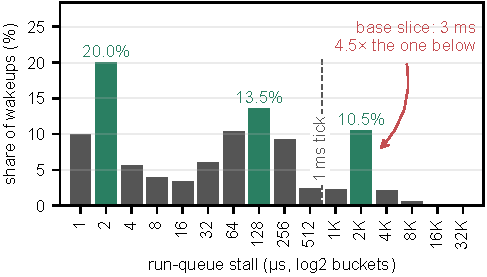
\includegraphics[width=\columnwidth]{docs/results/figures/stall_spectrum.pdf}
\caption{\textbf{Traced run-queue stalls are trimodal.} $\tracedEvents$
wakeups, \texttt{bpftrace} log$_2$ buckets, modes shaded. The jitter core peaks in the
$\tracedModeLoA$--$\tracedModeHiA\,\mu$s bucket, which alone holds $\tracedModeShareA\%$ of all
wakeups; a second mode at $\tracedModeLoB$--$\tracedModeHiB\,\mu$s holds $\tracedModeShareB\%$; the third, at
$\tracedModeShare\%$, lands on the scheduler's derived base slice of
$\baseSliceMs$~ms. A power law of any index above one would have to descend monotonically
across this axis. The count survives a
$\stallCoarsenFactor\times$ widening of the buckets in both phasings, so it is not an
artifact of where this tool put its edges.}
\label{fig:spectrum}
\end{figure}

That mode is the preempted state of Section~\ref{sec:mixture}, at a scale the scheduler's own
maintainers had already named: with run-to-parity a task's lag is held within
``$[-(\mathrm{slice} + \mathrm{tick}) : (\mathrm{slice} + \mathrm{tick})]$''~\cite{guittot2025slice}.
The histogram adds that this is where a tenth of all wakeups land, not merely a worst
case. The slice is \emph{derived} rather than measured: the kernel's published
rule~\cite{zhou2025slice} gives $\sliceFactor \times 0.75\,\mathrm{ms} = \baseSliceMs$~ms
on the $\testbedCpus$ cores the campaign's own load geometry recovers, over a $\tickMs$~ms
scheduler tick, and no scheduler tunable is written anywhere in the archived campaign
(Supplement~S16). That tick is the kernel's timer period, not the timestamp resolution $\tau$ of
Section~\ref{sec:metrics}; both are $1$~ms here by coincidence of configuration. A thread
descheduled at the wrong instant therefore reads its clock about a slice late, six to
thirty times a $0.1$--$0.5$~ms delivery, and the tick is why the mode is a band rather
than a spike. A mean over this distribution is dominated by a mode the operator never
sees, so a mean-based counter cannot flag this failure.

\section{Failure Mode 2: Quantization and Silent Deletion}
\label{sec:external}

The cross-broker benchmark we audit computes its reported latency distribution from a
subset of the samples it collected, does not record how large that subset was, and lets the
send rate decide it. Everything measured below is the
OpenMessaging Benchmark in embedded mode, where driver and workers run in one JVM. Its
distributed mode is discussed in Section~\ref{sec:limitations}.

\subsection{The admission condition, and its origin}
\label{sec:extmethod}
In \brk{LocalWorker.java}:294 the end-to-end latency is \texttt{now - publishTimestamp},
where \texttt{now} is read in the consumer and \texttt{publishTimestamp} is \kafka{}'s
producer-set \texttt{CreateTime}, itself a millisecond value. That difference is then
promoted to microseconds (Supplement~S25 quotes the call). A sample then enters the
histogram only if it passes the test in \brk{WorkerStats.java}:95 ---
\texttt{if (endToEndLatencyMicros > 0)} --- which we call the \emph{admission condition}.
The message is counted as received a few lines earlier, but a non-positive latency is
dropped and no counter records how many. Over the campaign of Section~\ref{sec:extphase}
that silence covers $\ombDiscarded$ samples.

The condition's origin is documented and its reasoning is sound. It was added in 2018 to stop
negative values reaching the histogram, on the ground that end-to-end latency ``is
calculated based on time difference of \texttt{System.currentTimeMillis()} on two different
machines'' and ``can be negative''~\cite{openmessaging_pr56}. The recorder is an
\texttt{HdrHistogram} \texttt{Recorder}, which rejects negative values outright, so
filtering for positives is the reasonable local fix, defensive rather than evasive. Its
non-local consequences are two, neither considered at the time. First, \texttt{> 0} also deletes
every sample that computes to exactly zero. Because
\texttt{System.currentTimeMillis()} has millisecond resolution, any delivery faster than
one millisecond does compute to zero. On co-located paths, where our own transport measures
$0.1$--$0.5$~ms, that is most of them. Second, the one observation which would show the
measurement had failed is the exact observation the condition removes.
Section~\ref{sec:tools} finds the same disposal, uncounted, in
\harnessSilentIndependentWord{} independent tools.

The condition's scope is telling. It is on the \ombGuardedPath{} path, which timestamps in
\ombGuardedClock{}s; the same harness measures its \ombUnguardedPath{} span with a
\ombUnguardedClock{} clock and records every sample unconditionally. The coarse clock and
the filter both landed on the one span that crosses processes.

\paragraph{The consequence, measured}
Of the $\ombMedianCells$ instrumented cells whose own summary we captured,
$\ombGridMedianCells$ report a median of $1.0$ or $2.0$~ms, and across those the benchmark
computes its reported distribution from between $\mathbf{\ombGridRetentionMin\%}$ and
$\mathbf{\ombGridRetentionMax\%}$ of the samples it takes. Two replicates of one cell ---
$200$~B payload at $500$~msg/s, same host --- kept $\ombKeptLo$ and $\ombKeptHi$ samples, a
$\ombRetentionFold$-fold difference, and both reported a median of $1.0$~ms with nothing in
the output to distinguish them. Three uninstrumented runs print p50, p95, p99 and max all
equal to $1.0$ to three decimal places. The full ledger holds $\ombRuns$ instrumented runs,
$\ombDiscarded$ discarded samples and $\ombNegatives$ negatives, and over it the retained
fraction falls as low as $\ombRetentionMinExact\%$ --- four samples kept of ninety thousand.
The printed median is pinned at the timestamp resolution while retention moves across two
and a half orders of magnitude (Fig.~\ref{fig:deletion}). The only cells that escape are the four whose payload is large enough that
the resolution stops binding.

That discarded fraction is the one time-interval averaging measures
with~\cite{hp1970tia}: reporting a distribution conditioned on it, without reporting it,
keeps the residue and throws away the estimator.

\begin{figure}[tb]
\centering
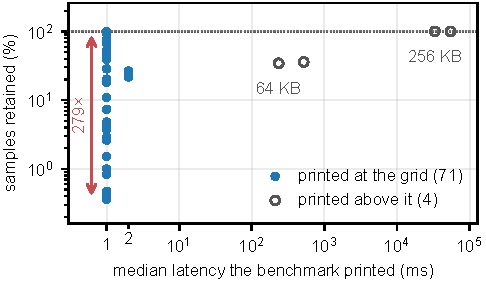
\includegraphics[width=\columnwidth]{docs/results/figures/deletion.pdf}
\caption{\textbf{What the benchmark prints against what it kept in order to print it}, over
the $\ombMedianCells$ cells that printed a summary of their own. At the timestamp resolution the printed median carries no
information about retention: $\ombGridMedianCells$ cells report $1.0$ or $2.0$~ms while the
retained fraction spans $\ombRetentionFold\times$. Away from it the harness behaves: the
failure is confined to deliveries shorter than the timestamp resolution.}
\label{fig:deletion}
\end{figure}

\subsection{Phase, and the grid it produces}
\label{sec:extphase}
Publish latency across these cells takes only two values, $\ombPubLatLo$ and
$\ombPubLatHi$~ms, while retention varies $\ombRetentionFold$-fold. A two-valued predictor
cannot account for a range like that whatever its correlation, and the correlation it does
have ($\ombRetentionRho$, Fisher $\ombRetentionRhoCI$, over $\ombRetentionRhoN$ cells) carries
the sign the law below predicts. What moves retention is where the producer's send
instants fall against the \emph{grid}: the instants, one millisecond apart, at which the
timestamp changes value. A sample survives when its delivery crosses a grid instant,
which for $T_{\mathrm{true}} < \tau$ happens with probability $T_{\mathrm{true}}/\tau$
(Supplement~S17 draws the geometry):
\begin{equation}
\label{eq:retention}
\text{retention} \;=\; \min\!\left(1,\; \frac{T_{\mathrm{true}}}{\tau}\right)
\qquad\text{(uniform phases).}
\end{equation}

All \spreadIncommensurateWord{} configurations whose send interval is incommensurate with
$\tau$ sit near $50\%$ --- medians $\spreadIncommensurateLo$ to
$\spreadIncommensurateHi$ --- implying $T_{\mathrm{true}} \approx 0.5$~ms at
$\tau = 1$~ms.

\paragraph{A pre-registered confirmation}
\label{sec:extcomp}
Payload moves $T_{\mathrm{true}}$, and with it the fraction a run retains. Where the send
interval is commensurate with the tick the retained fraction is confined to a few values
rather than a continuum, so moving $T_{\mathrm{true}}$ moves a configuration between them.
Supplement~S10 sets that structure out and draws all three payloads against it; S11 tests it
configuration by configuration against the permutation null S14 constructs. The prediction was registered before the runs and it came
true: replicate spread collapses to $\flipSpreadThirtyTwo$ points at $32$~KB and re-opens
to $\flipSpreadSixtyFour$ at $64$~KB, a
boundary crossed in both directions by one manipulated variable. One registered detail
failed --- the $32$~KB configuration pins at $\flipPinThirtyTwo\%$ retention, not on the predicted
vertex at $\flipVertexTwoThirds\%$ ---
% The payload-flip figure moved to the supplement in round 43, beside S10, which is where
% the spread rule it confirms is set out in full. Same journey as the pipeline schematic in
% round 16 and the payload-sweep law earlier in this round, and for the same reason: every
% number the panels carry is in the sentence above them, so the figure restates rather than
% shows, and four biographies would not otherwise fit inside twelve pages.

% Round 47 cut the sixty-three-cell campaign's tally to its conclusion. It was two sentences
% of tier-4 evidence -- six registered predictions, three falsifiers fired -- and S7 gives
% every one of them prediction by prediction, so the main text was carrying an index to a
% table rather than a result. The page it bought went to the two citations round 46 asked
% for, one of them a paper in this journal on this section's own subject.
and a larger campaign leaves per-send jitter rather than accumulation standing
(Supplement~S7).

\subsection{Our own harness, and the sign channel}
\label{sec:generality}
To show the deletion is not an artifact of one JVM, we reproduced the admission condition in an
independent Python harness sharing no code with the benchmark. On one clock it recorded
\textbf{zero} negative differences across $\harnessOneClockSamples$
samples, as a causal chain requires, and none across two hosts either
(Supplement~S22). The grid behavior reappeared intact. At
$\harnessXHostRate$~msg/s --- the \harnessXHostArmClass{} configuration, the only one of the
three whose own grid spread does not swamp the comparison --- cross-host retention wandered
from $\harnessXHostRetLo$ to $\harnessXHostRetHi\%$ over four replicates, where the same
configuration on one clock held to $\harnessOneClockSpread$ points.
Cross-host, the deleted fraction couples to the synchronization state and nothing records
either. 

Separating the discards by sign is what makes the condition's cost legible. Across the
\kafka{}-driver corpus's $\ombKafkaRuns$ runs its $\ombKafkaDiscarded$ discarded samples
contain \textbf{not one negative}: the most negative value at any load, size or rate is
$0\,\mu$s.
Those discards are resolution failures, not clock failures --- a distinction an unsigned
counter cannot make. The same channel
then caught the real thing in the \redis{}-driver replication's $\ombRedisRuns$ runs:
$\ombRedisNegatives$ negatives, every one exactly $-1000\,\mu$s, the smallest value a
one-millisecond timestamp can express, with
$\ombRedisWorstNegatives$ of them in a single run where they were \emph{half of all samples
taken}, beside \ombRedisWorstKept{} kept.

That value is not a coincidence. The \redis{} driver's span is a difference between two
millisecond-floored clocks on two hosts, and a sub-tick offset between two floored clocks can
produce exactly one negative value, $-1000\,\mu$s, and no other. That is precisely what the
corpus contains. The \kafka{}-driver span, floored the same way but taken inside one
JVM, never inverts at all. Clock discipline was clean at every logged minute, which is the
point --- this failure needs no misbehaving clock, only two of them and a floor
(Supplement~S14).

\section{Evidence Across Tools}
\label{sec:tools}
% Round 60: the fork count used to open this section, and a fork is a copy -- the number
% bounds how few have diverged, not how many adopted. The audit below is the independent
% evidence, and it is the one with a registry behind it, so it opens instead.
The disposal is a pattern across the tooling rather than one project's oversight.
We audited \harnessAuditedWord{} tools at source
across \harnessLanguagesWord{} languages and \harnessVendorsWord{} vendors, classifying each
% Lower-case twin, not the ...Cap one: round 61's reordering put this clause after a
% semicolon rather than at the head of a sentence. Lesson 12 in reverse.
finding with the code that classified the benchmark; \harnessSilentWord{} of the
\harnessAuditedWord{} dispose of the sample without counting it, in
\harnessDisposalClassesWord{} classes, and one of them reaches that class at the other
threshold. Apache Pulsar's performance client admits zero~\cite{pulsar_perf}, so it drops the
negative spans and keeps the sub-resolution samples the benchmark deletes. They survive into
its output, where an operator can see them pile up on the quantum. Deletion is not the only way coarse resolution wins: Apache
\kafka{}'s own bundled end-to-end tool keeps every sample and loses it anyway, filling the
array its percentiles come from by integer division, so on a sub-millisecond path every
one reports zero~\cite{kafka_tools}. Two more keep their negatives and pass them on
unfiltered, as RFC~7679 asks~\cite{rabbitmq_perftest,nats_cli}. The failure is not universal,
and the claim that survives is the narrower one: \emph{the tools that quantize or filter do so
without counting}. Substitution is the worst of the three classes because it leaves
nothing missing: \texttt{fio} and \texttt{btt} substitute zero and one nanosecond, and a
value never measured enters the distribution. At the other end, \harnessCountingWord{} counts
its discards in a metric whose description names the cause~\cite{rezolus}, which is what
makes the rule of Section~\ref{sec:authors} practical rather than aspirational.
Supplement~S25 gives the registry tool by tool, with the source line each finding sits on and
one entry that corrects a misreading of our own. The class is not confined to benchmarks:
in November 2025 the audited broker's own coordinator metrics adopted the same disposal,
clamping negative durations to zero with no counter~\cite{kafka19888} (Supplement~S25).
The admission condition also survives downstream: $\forkUnchanged$ of the $\forkChecked$
public forks we could read carry the expression unchanged (surveyed \forkCheckedOn{}), which
bounds how few have diverged rather than how many chose it.

\section{Discussion}
\label{sec:discussion}
Both failures are cheap to detect and neither is detected, so the remedy is a reporting
rule rather than a better clock.

\subsection{What the brokers actually do}
\label{sec:brokers}

Once the failed runs are removed, the broker comparison that motivated the work is small and
one configuration choice dwarfs it. On gated artifacts the two sit within a millisecond on
the transport proxy (TOST against a $\tostMargin$~ms margin, $p < 0.001$, across
$\tostLevels$ levels), so it is not a purchasing argument. The one condition that reverses
the ordering is a consumption pattern rather than the broker, and a co-located testbed ---
the standard evaluation environment --- hides it (Supplement~S13).

Our own measurement is not symmetric across that comparison, and the rule below says to
declare it: \kafka{}'s client deserializes the payload before $t_{\mathrm{recv}}$ and
\redis{}'s after it, worth $\spanHandlingWorstUs\,\mu$s or $\spanHandlingSharePct\%$ of
\redis{}'s median delivery. That is a fiftieth of the equivalence margin, it runs
\emph{against} the per-broker difference of Table~\ref{tab:spans} rather than producing it,
and \tti{} is free of it (Supplement~S16.1).

\subsection{For benchmark authors}
\label{sec:authors}

SPEC and TPC judge a benchmark on five criteria~\cite{kistowski2015build}. The tool we
audit passes the half of \emph{reproducibility} a reader checks ---
run-to-run consistency at a fixed configuration --- \emph{because} it fails
\emph{verifiability}. A median from $\ombGridRetentionMin\%$ of the samples is the more
stable for having had the variation deleted, and a second tester who picks a different send
rate measures a different sample. Every rule below instances the criterion that can see this.

\textbf{Report a physical-consistency audit.} Any cross-process timestamp difference admits
a sign check that costs nothing, and every run it rejected here had passed every conventional
check we knew. Better measurement systems
exist~\cite{yang2022cloudprofiler,kogias2019lancet,kundel2024p4sta}; whatever the
measurement, check its output against causality and publish the rejection rate, as network
clocks have for thirty years~\cite{paxson1998calibrating,paxson2004sound}. The discipline is tested only by a
campaign the rate costs something, and ours cost us a result.

\textbf{Say which physical event each timestamp marks.} A timestamp is a clock read,
not the event it stands for, and the gap between them is where both failures live. Publish
where in the code each one is taken and what has already happened when it runs: our own two
clients differ by a payload parse (Supplement~S16.1), and no reader could have known.

\textbf{Name the span you are subtracting.} A difference of two timestamps is a latency only if
the first event causally precedes the second. An acknowledgment at the producer does not
precede a record at the consumer (Section~\ref{sec:proxy}). We caught our own instance
only on counting the send-referenced span separately (Table~\ref{tab:spans}).

\textbf{Where the span cannot be re-timestamped, recover the displacement rather than
discard it.} A harness that records its own acknowledgment lag recovers the delivery it
failed to measure, on the runs the check rejects as well as on those it passes
(Section~\ref{sec:cost}). This does not reopen the gate of Section~\ref{sec:gate}: that rule
declines to publish the proxy as a latency, and this one reports the delivery instead.

\textbf{Two delays with one cause are not independent.} Timestamps waiting on one scheduler move
together (median correlation $\spanRhoMedian$), so multiplying their probabilities
misprices the answer.
Assuming independence here overpredicts the negative-span rate in all $\indepConditions$
conditions, by a median factor of $\indepOvershoot$.

\textbf{Know where your own path sits on the exposure curve, and how wide it is.} The
relative error of an acknowledgment-referenced span is $A/D$ (Section~\ref{sec:cost}).
Measure your own $A$: ours spans an order of magnitude across conditions and moves the
crossover with it. A harness that subtracts a send timestamp is not on the curve at all, which is the
whole return on naming the span.

\textbf{Count your events before you quote a percentile.} A median over as few as seven
events per run is not a property of the system, and repetition will not tell you so.

\textbf{Exercise the timestamping path at the load you will report from.} A path that
is clean idle is not thereby clean at the knee: the same threads on the same host move the
negative-span rate $\rtFactorLow$--$\rtFactorHigh\times$ between priorities, and the rate
we measure at $88\%$ is $\diseaseOverWhole\%$ of events. Run the sign check under the load
the numbers will be quoted at, not under a quiet one.

\textbf{Make the timestamping path unpreemptable, and say that you did.} The one mitigation
our measurements support directly: real-time priority on the timestamping threads cut the
negative-span rate $\rtFactorLow$--$\rtFactorHigh\times$ at unchanged background load.
Busy-polling a dedicated core should buy the same for the price of that core, though we did
not measure it. Two caveats: the floor is not zero, so the check stays. And a real-time or
polling timestamping thread changes the system it measures, so where that is unacceptable,
report retention instead.

% Worded to match the abstract's closing sentence verbatim: this is the same rule and a
% reader should be able to quote it once. The defined term stays two lines below, where
% Section III's definition governs it.
\textbf{Dither the send instant, and publish the retained fraction.} Randomizing probe timing
to avoid synchronizing with a periodic phenomenon is long-standing
advice~\cite{rfc2330,rfc3432}, and the counter literature that carries our retention
identity~\cite{hp1970tia} already names the coherence it breaks. What we add is what it
costs when the samples are deleted rather than averaged. Publish beside the latency the retention rate, the timestamp
resolution and the synchronization state, none recoverable afterwards. A summary from
$\ombGridRetentionMin\%$ of samples is typographically identical to one from all.
Neither half of the rule is ours: OWAMP has attached an error estimate to every timestamp
since 2006, and records a packet timestamped in the future unaltered rather than discarding
it~\cite{rfc4656} (Supplements~S31 and~S32 give the precedents). The sign is the channel:
negative means the reference timestamp failed, computes-to-zero means the resolution
failed, and one unsigned total cannot distinguish them.

\textbf{Do not assume co-location makes the measurement safer.} One host removes the
clock-synchronization rival and nothing else: \brk{mq-bench} below gives co-location as the
reason its timing is sound, and is sound for a different reason it does not state
(Supplement~S33.3). The configuration our audit rejects most often
is co-located, it hid the one condition that reverses our broker ordering
(Section~\ref{sec:brokers}), and a shorter path is exactly the path on which both failures
bind hardest.

\textbf{Record the achieved rate, not the flag meant to produce it.} Verify it per run against
elapsed wall time. The send schedule is an experimental variable in
Section~\ref{sec:external}, not a nuisance parameter. We found runs where configured
and achieved rates disagreed.

% Round 54 (M5a): "a 2026 framework" and Section III-A's "2026 comparison" are different
% objects, and a reader meeting the second had no way to tell. Naming this one settles it,
% and costs no reference: the supplement cites mq-bench where the bibliography is uncapped.
None of this is hypothetical: \brk{mq-bench}, a 2026 framework for the same comparisons,
already timestamps in nanoseconds and subtracts a span that cannot invert, both choices made
and neither argued for (Supplement~S33.3). Nor is it unwelcome. The tool we audit
accepted a coordinated-omission report and now records the publish delay, and the
admission condition came through that revision untouched. A later request would
serialize the histograms it discards after reading their summaries; that export
carries the deletion into a new container unless the retained fraction travels with
it (Supplement~S22).

\subsection{The limits of a better clock}
\label{sec:betterclock}
Hardware-timestamped PTP~\cite{ieee1588} would take two LAN hosts from our
$\interHostOffsetUs\,\mu$s of \texttt{chrony} agreement to sub-microsecond. Behind a
one-millisecond timestamp, $\interHostOffsetUs\,\mu$s and $70$~ns produce byte-identical
records. The admission condition deletes the same samples and the retention arithmetic is
unchanged.
The remedies are therefore ordered:
record at native resolution, count what is discarded, dither the send instant, and only then
is synchronization quality the frontier (Section~\ref{sec:generality}).
% Round 47 cut the redesign clause to its pointer. That a consumer-to-producer acknowledgment
% removes skew but not this failure, and that every one-way-avoiding scheme rests on an
% unstated assumption, are both worked through in S29 and S16.5; the main text needs the
% conclusion, which is the last sentence of this paragraph.
Resolution is the lesser half, and a distinct one. A microsecond timestamp retires
Equation~\ref{eq:retention}'s deletions here and moves the grid to faster paths, but the
admission condition and genuine negatives survive it (Supplements~S29 and~S16.5). A better
clock alone therefore converts an uncounted \emph{resolution} failure into an uncounted
\emph{timestamping} one.

\subsection{Threats and limitations}
\label{sec:threats}
A negative span shows that the acknowledgment cannot serve as the origin of a delivery
latency for that event; attributing that to scheduling is an inference, separated from its
rivals by manipulation, with the eliminations listed below. Beyond that list, the
clustering of consecutive late wakes
($z = -6.9$ at the co-located floor, at every load including none) is the signature of a
shared scheduling delay, not independent kernel granularity. The \texttt{chrony} daemon
reports the inter-host offset as comfortably sub-tick but bounds its own error at
$\chronyHostBoundLo$--$\chronyHostBoundHi$~ms per host; the two worst bounds sum to
$\chronyPairBound$~ms against a $1$~ms timestamp, so the cross-host channel stays open
rather than ruled out. It did not produce the \redis{}-driver
negatives, which the driver's own timestamp accounts for exactly
(Section~\ref{sec:generality}), but it is why we claim no cross-host bound in general. The
skew threshold of Section~\ref{sec:related_time} does not transfer to a loaded machine
either (Supplement~S33).

\label{sec:limitations}
\paragraph{Scope, and the alternatives eliminated} Three widely used runtimes document this structure without drawing its consequence for a
cross-process subtraction (Supplement~S30).
The mechanism requires a timestamping path that can be preempted. Designs that pin a thread to
a dedicated core and busy-poll, or that timestamp in hardware, remove the preempted
state the mechanism depends on, and we make no claim about them. Within our own
setting the alternatives are each eliminated. Clock skew: one clock by
construction on the rejecting configurations, and $\harnessCrossHostNegatives$ negatives in
$\harnessCrossHostSamples$ two-clock samples. Cross-CPU incoherence under migration: below. Utilization: identical
$\rho$, rates twofold apart. Timer noise: \texttt{SCHED\_FIFO} at fixed utilization
collapses the rate across $\rtPairs$ pairs, and noise does not respect
scheduling class. Stress: transport $\payloadTransportFactorRound\times$ longer
\emph{lowers} the rate. Direct observation: a
\brk{sched_switch} histogram predicts the rate to within a third, unfitted. One rival is
not the scheduler's --- the timestamp is a CPython call, so it waits on the interpreter lock
too, invisibly to a tracepoint probe. That one is bounded because the kernel-only estimator
brackets the observed rate ($\tracedRatios$) instead of under-predicting (Supplement~S16.4).

% Round 47 tried to compress this paragraph for the page budget and put both of its pinned
% clauses back. "both of which" is the plural antecedent for the two admitted clocksources,
% and "on headroom, not on shared endpoints" is the only visible trace of an argument this
% paper abandoned -- an early version reasoned from the shared closing clock read, which does
% not discriminate. Two tests hold them; the words for the budget came from elsewhere.
Clock incoherence across vCPUs, our machines being virtual~\cite{kvmclock}, is closed
twice. The probe's $\clockIncrementNs$~ns increment admits only
\clockAdmitted{}, both of which the kernel uses solely where cross-CPU coherence is
asserted; and the corpus closes the channel again on headroom, not on shared endpoints, since
the send-referenced span holds a floor $\spanOffsetMargin\times$ too high to explain the
deepest negative span (Supplement~S15).

The mechanism's constants are those of one EEVDF-era kernel (6.8); CFS-era schedulers, the
regime Lozi et al.\ document, may shift them. The deletion arithmetic is demonstrated on one
benchmark and reproduced in one independent harness. The \harnessAuditedWord{} tools of
Section~\ref{sec:tools} are readings of source rather than measured deployments, and are
exact to the threshold rather than to the behavior a deployment would show. The
benchmark's distributed mode failed on every attempt, so its cross-host exposure rests on
source reading and our own two-host harness (Supplement~S24). Exposure depends on a
deployment's path latency and producer rate. That is why we recommend publishing a
retention rate rather than calling any published number wrong.

\section{Conclusion}
\label{sec:conclusion}

A latency benchmark measures the system only while its timestamps are taken faster than
the delivery it measures. Below that line the two failures reported here appear, invisible
in the output. Two timestamps written by threads that each wait for a core on their own
account invert the delivery between them whenever those waits differ by more than it. A timestamp quantized
to a millisecond, filtered for positivity, deletes most of a sub-millisecond path by
arithmetic the operator never sees. Neither needs a better clock, and neither is expensive
to detect. Check the spans whose endpoints are timestamped in different places, count what
your tool throws away, and publish the retention rate beside the number.

% Four correspondents were thanked here by name until 2026-09-10, when all four were cut
% under one rule: a paper thanks the people who are still in the conversation, and none
% had written since August. What they gave is still in the paper -- the same-clock
% contrast, the kernel-tracing pointers, the probe-placement argument and the resolution
% question all shaped sections that remain -- and the citations they led to are unchanged.
%
% N. Herbst is back, on the same rule rather than an exception to it. He asked on the 10th
% to come off the byline, was asked whether he would still take an acknowledgment, and
% answered the same day that he would. The other three have not written since August and
% stay out; if any of them writes, the rule puts them back too.
%
% The disclosure paragraph is not optional: IEEE requires it for generative-AI assistance.
% R4 (round 66) asked whether this heading should read "Disclosure", since the
% section now holds only the generative-AI statement and a reader meeting
% "Acknowledgment" expects thanks. It stays. IEEE's own template names this
% section, its generative-AI policy puts the disclosure inside it, and the
% paragraph says what it is in its first five words, before the friction can
% build. scripts/build_without_authors.py and three gates key on the heading.
\section*{Acknowledgment}

The authors thank N.~Herbst, for the load-generation point that became one of the
reporting rules above, for the timer-characterization work cited in
Section~\ref{sec:related}, and for a reading that reset the abstract.

In accordance with IEEE policy, Anthropic's Claude assisted with code development and
verification, manuscript editing, and literature search. Experimental design, scientific
claims, and interpretation are the authors'.

\section*{Artifact Availability}

% Concept DOIs, not version DOIs. A Zenodo concept DOI is stable across every version and
% resolves to the newest; the version DOIs printed here until v2.5 pinned a record that the
% next deposit superseded, so a reader of the current paper was sent to the previous archive.
% The version is named so the record this PDF sits in is still identifiable --
% and is EMITTED from .zenodo.json rather than typed, because when it was typed
% it named v2.6.0 from inside the v2.7.0 archive, which is the one failure the
% sentence exists to prevent.
Code, analysis and manuscript are archived at
\href{https://doi.org/10.5281/zenodo.21650031}{10.5281/zenodo.21650031}, the measurement
dataset at \href{https://doi.org/10.5281/zenodo.21650064}{10.5281/zenodo.21650064}; both
resolve to the current version, \texttt{v\artifactVersion}, whose files are
\artifactAccessPhrase{}. Every
number here is recomputed from the committed data by the archived code at build
time, and the test suite fails if the text and the data disagree.

\bibliographystyle{IEEEtran}
\bibliography{manuscript_references}

\begin{IEEEbiographynophoto}{Gustavo Pedro Ricou}
% Trimmed twice: once when the author list went from two names to four, and again in round
% 43, when four biographies would not fit inside twelve pages. What went the second time:
% "with first-class honors", the specialization venues, and one clause of the research line.
%
% Round 45 trimmed it a third time for the page budget and put every word back. Three of the
% clauses it cut are pinned by tests, each for a reason recorded when it was pinned: "with
% first-class honors" and "currently pursuing" because an earlier draft understated the
% degrees held and blurred the one in progress, and "pre-registration" because the research
% statement has to describe a programme rather than this paper. A page budget is not a reason
% to reopen a decision about how a person's own record is stated; the words were found
% elsewhere.
received the B.Sc.\ degree in physics from the Universidade do Porto, Portugal, and
specialized in nuclear fusion science at the Universit\"at Stuttgart, Germany, and the
Universit\'e de Lorraine, France. He holds an
M.Sc.\ in software design with cloud-native computing from the Technological University of
the Shannon, with first-class honors, and is currently pursuing an M.Sc.\ in statistics and
data science at Trinity College Dublin, Ireland. He is a Software Engineer with
BoscaSports. His research concerns measurement validity --- what a reported number is really
evidence of --- in computer systems, environmental measurement and sports analytics, using
pre-registration and physical-consistency auditing.
\end{IEEEbiographynophoto}

% DUVIGNAU: CONFIRMED BY HIM on 2026-09-04. The entry was drafted from his own public
% pages (chalmers.se/en/persons/duvignau and cse.chalmers.se/~duvignau, read 2026-09-02)
% under the rule used for all of them -- draft it from the public record so the person's
% task is CORRECTING rather than writing -- and he returned it with one change: the unit
% is the NETWORK AND SYSTEMS unit, not "Computer and Network Systems". The Chalmers page
% carries the longer name; he does not. His words win. That rule paid three times over
% four entries, two of which have since been withdrawn.
%
% WHY THERE ARE TWO BIOGRAPHIES. The paper carried four names until 2026-09-10. The last
% author withdrew on 8 September on his own standard for what he can take public
% responsibility for in a deposited record he has not audited; the third asked on the
% 10th for his name to come off the work entirely, having read the manuscript and passed
% it three days earlier, on an objection to how the work was produced rather than to what
% it reports. Neither withdrawal moved a number, a figure or a claim, and neither is a
% reason to delete what they contributed: the load-generator rule still closes the paper,
% the timer-characterization citation stays in Section III, and Figure 1, the thread
% drawing and the deletion histogram stay with the gates that pin them. Do not restore a
% byline from an old draft; tests/unit/test_front_matter_agrees.py pins it at two.
\begin{IEEEbiographynophoto}{Romaric Duvignau}
received the Ph.D.\ degree in computer science from the University of Bordeaux, France, in
2015, for work on the maintenance and simulation of dynamic random graphs. He is an
Associate Professor and Head of the Network and Systems unit at Chalmers
University of Technology, Gothenburg, Sweden. His research concerns distributed and
data-driven algorithms, the monitoring of large-scale distributed systems, and stream
analytics for cyber-physical systems.
\end{IEEEbiographynophoto}


\end{document}
